\documentclass[11pt]{article}

\usepackage{amsmath}
\usepackage{enumitem}
\usepackage{graphicx}

\title{ECS 152A Programming 2}
\author{
  Daniel Phan \\
  ID 914831996 \\
  Section A04
  \and
  Noah Tarr \\
  ID 917286014 \\
  Section A02
}
\date{Due: 03/07/2021}

\setlength{\oddsidemargin}{0in}
\setlength{\evensidemargin}{0in}
\setlength{\topmargin}{0in}
\setlength{\headheight}{0in}
\setlength{\headsep}{0in}
\setlength{\textwidth}{6.5in}
\setlength{\textheight}{9.25in}
\setlength{\parindent}{0in}
\setlength{\parskip}{2mm}

\begin{document}

\maketitle

\section{HTTP Wireshark Lab}

\subsection{The Basic HTTP GET/Response Interaction}

\begin{enumerate}
\item Is your browser running HTTP version 1.0 or 1.1?  What version of HTTP is
  the server running?
  \begin{itemize}
  \item Both my browser and the server are running HTTP version 1.1.
  \item 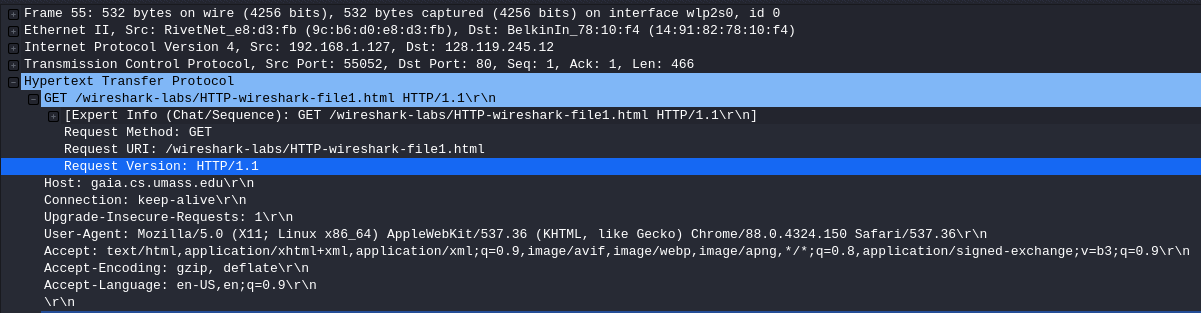
\includegraphics[width=\textwidth]{img/ws-browser-http-version}
  \item 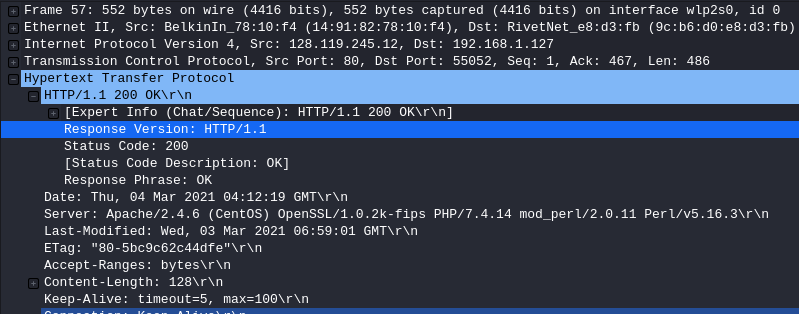
\includegraphics[width=\textwidth]{img/ws-server-http-version}
  \end{itemize}
\item What languages (if any) does your browser indicate that it can accept to
  the server?
  \begin{itemize}
  \item My browser indicates that it accepts US English.
  \item 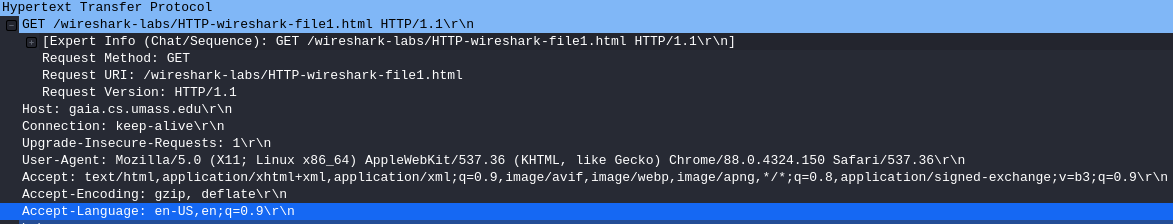
\includegraphics[width=\textwidth]{img/ws-browser-language}
  \end{itemize}
\item What is the IP address of your computer?  Of the gaia.cs.umass.edu server?
  \begin{itemize}
  \item My IP address is 192.168.1.127, while the server's IP address is
    128.119.245.12.
  \item 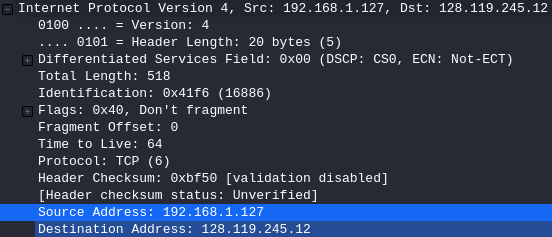
\includegraphics[width=\textwidth]{img/ws-my-ip}
  \item 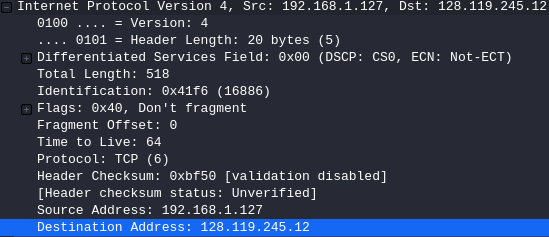
\includegraphics[width=\textwidth]{img/ws-server-ip}
  \end{itemize}
\item What is the status code returned from the server to your browser?
  \begin{itemize}
  \item The server returned $200$ for the HTML file and $404$ for favico.ico.
  \item 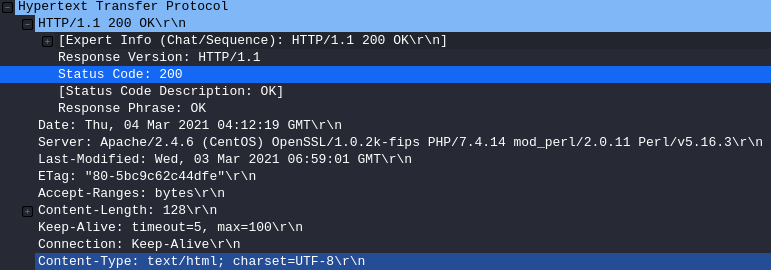
\includegraphics[width=\textwidth]{img/ws-status-code-1}
  \item \item 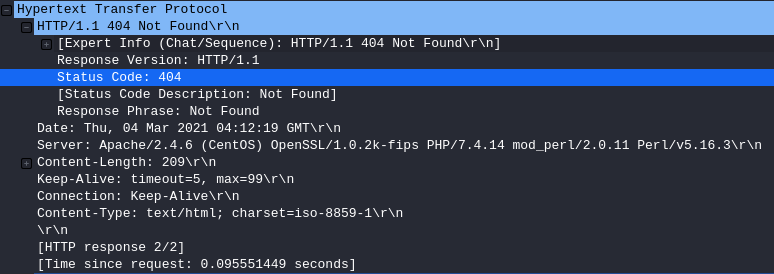
\includegraphics[width=\textwidth]{img/ws-status-code-2}
  \end{itemize}
\item When was the HTML file that you are retrieving last modified at the
  server?
  \begin{itemize}
  \item It was last modified on March 3, 2021, at 06:59:01 GMT.\
  \item 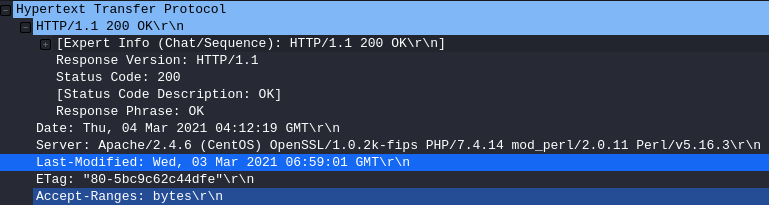
\includegraphics[width=\textwidth]{img/ws-last-modified}
  \end{itemize}
\item How many bytes of content are being returned to your browser?
  \begin{itemize}
  \item There were $128$ bytes for the HTML file, and $209$ bytes for
    favico.ico.
  \item 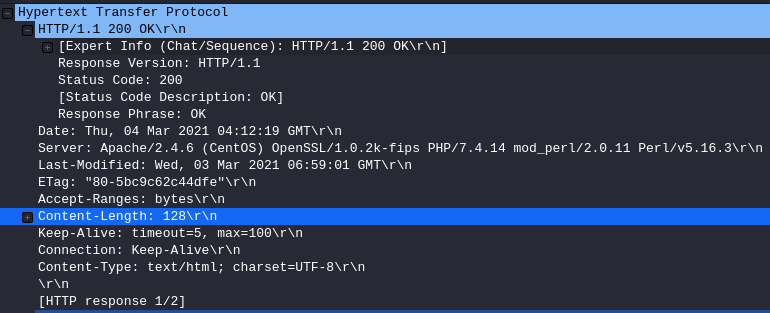
\includegraphics[width=\textwidth]{img/ws-content-size-1}
  \item 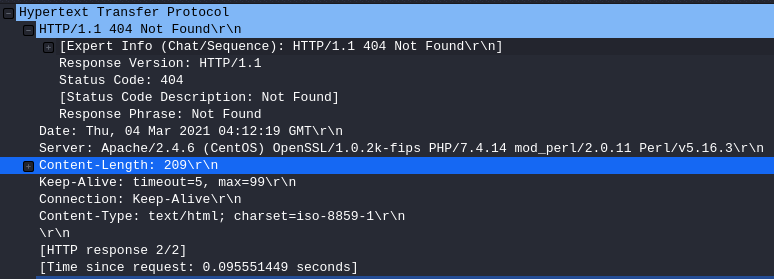
\includegraphics[width=\textwidth]{img/ws-content-size-2}
  \end{itemize}
\item By inspecting the raw data in the packet content window, do you see any
  headers within the data that are not displayed in the packet-listing window?  If
  so, name one.
  \begin{itemize}
  \item I do not see any headers that are not displayed.
  \item 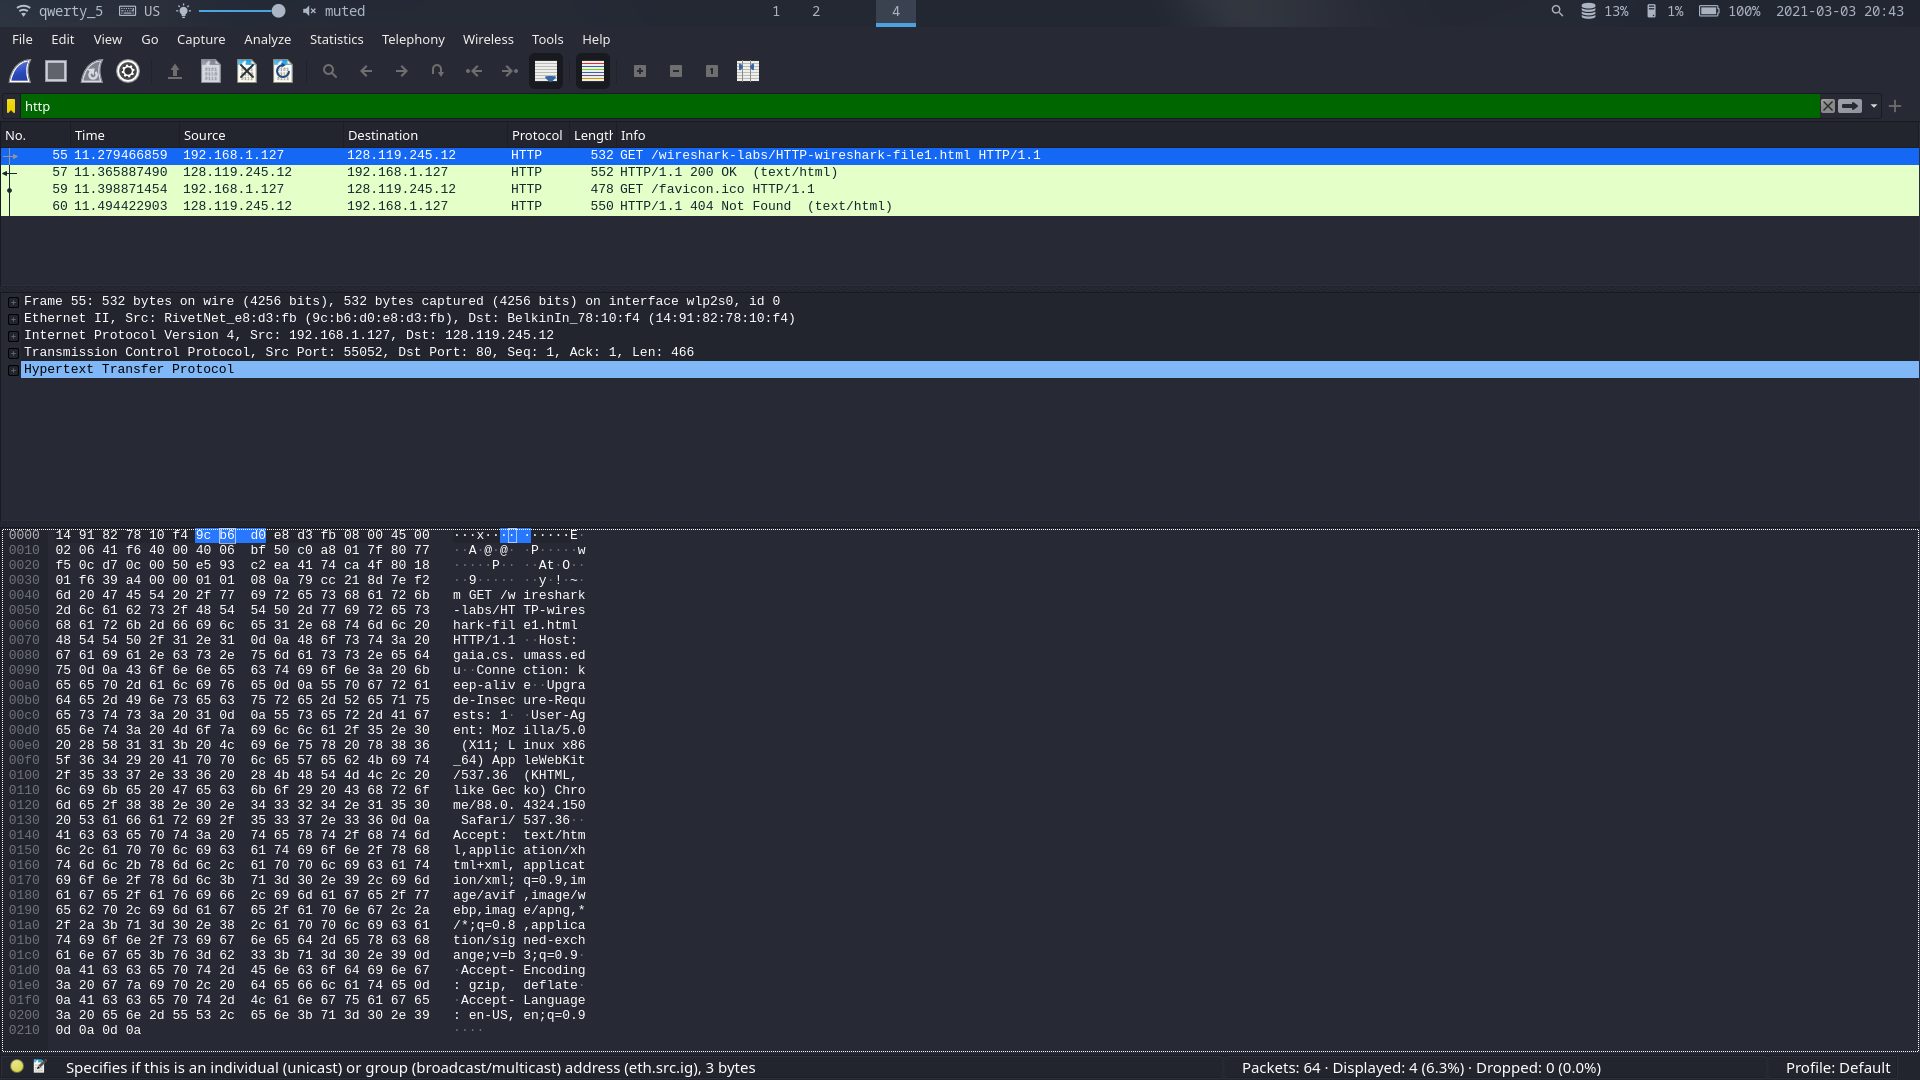
\includegraphics[width=\textwidth]{img/ws-raw-data-1}
  \item 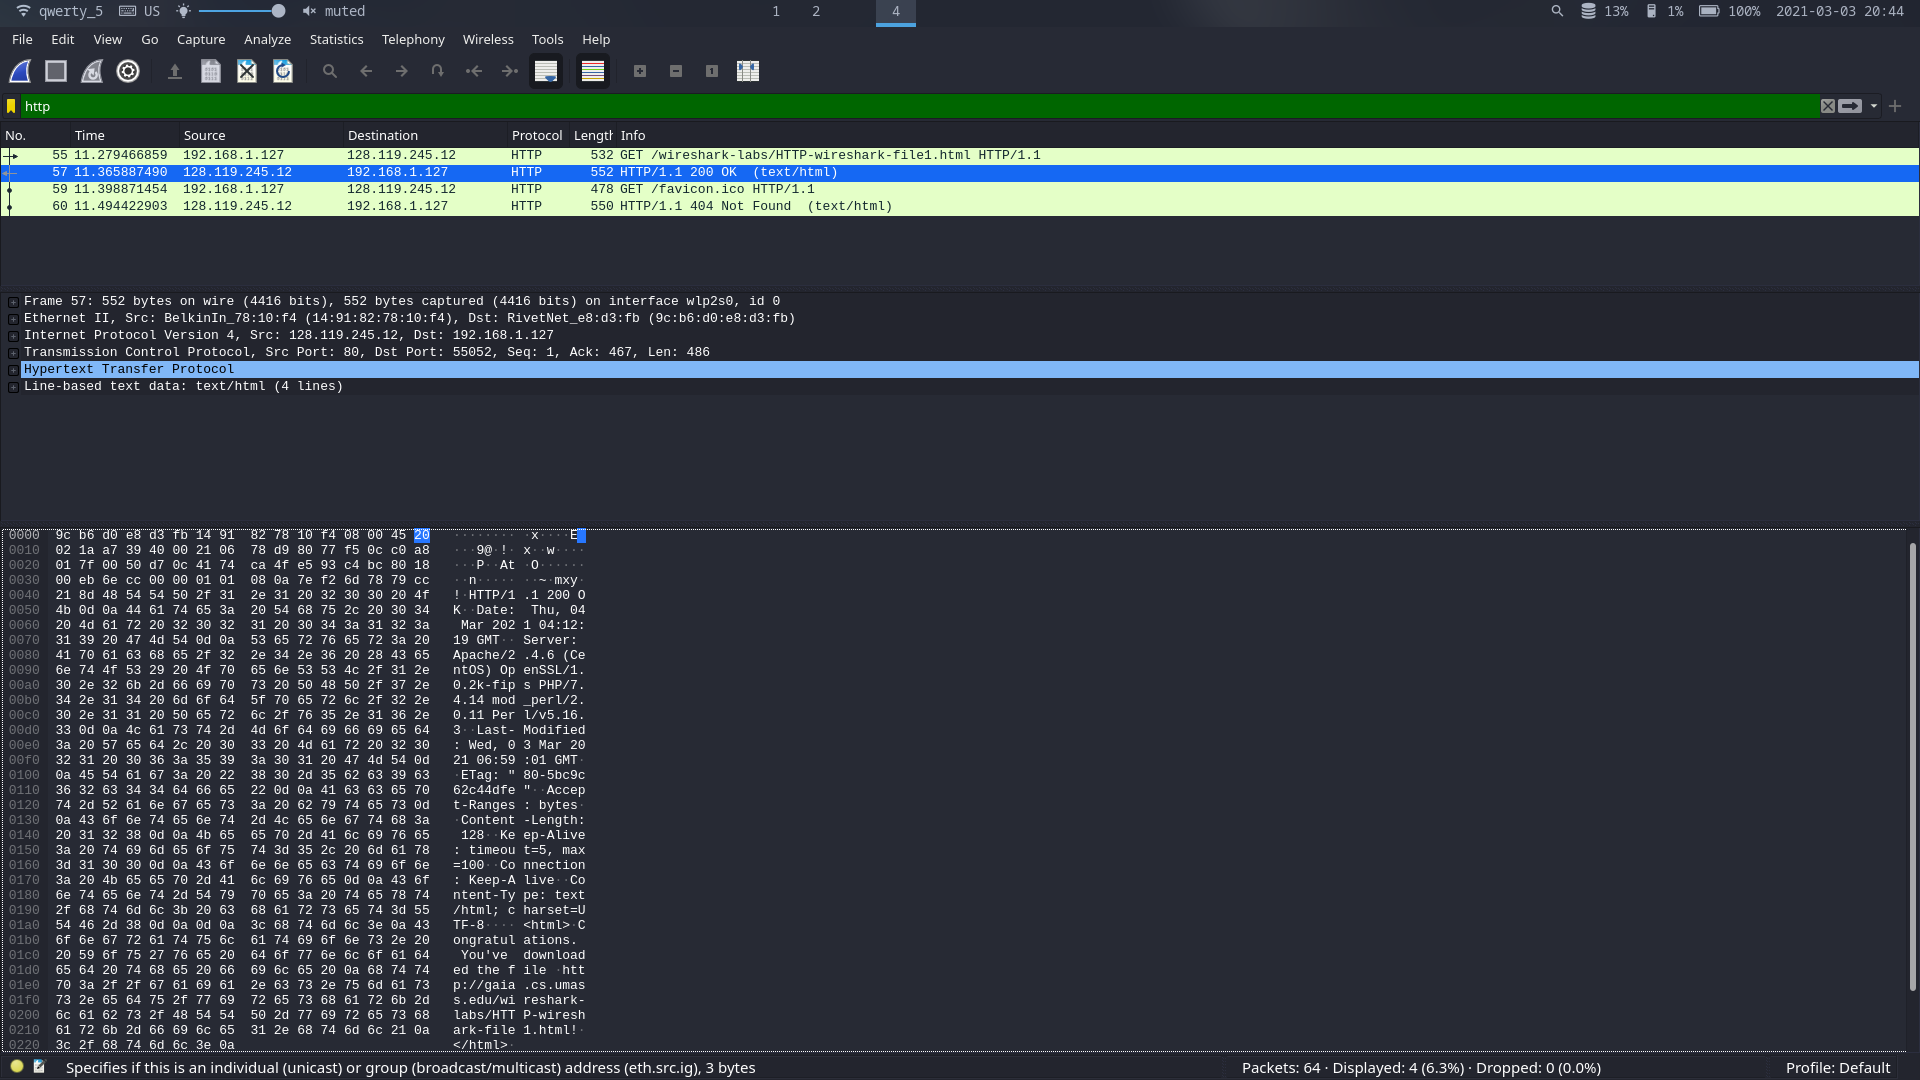
\includegraphics[width=\textwidth]{img/ws-raw-data-2}
  \item 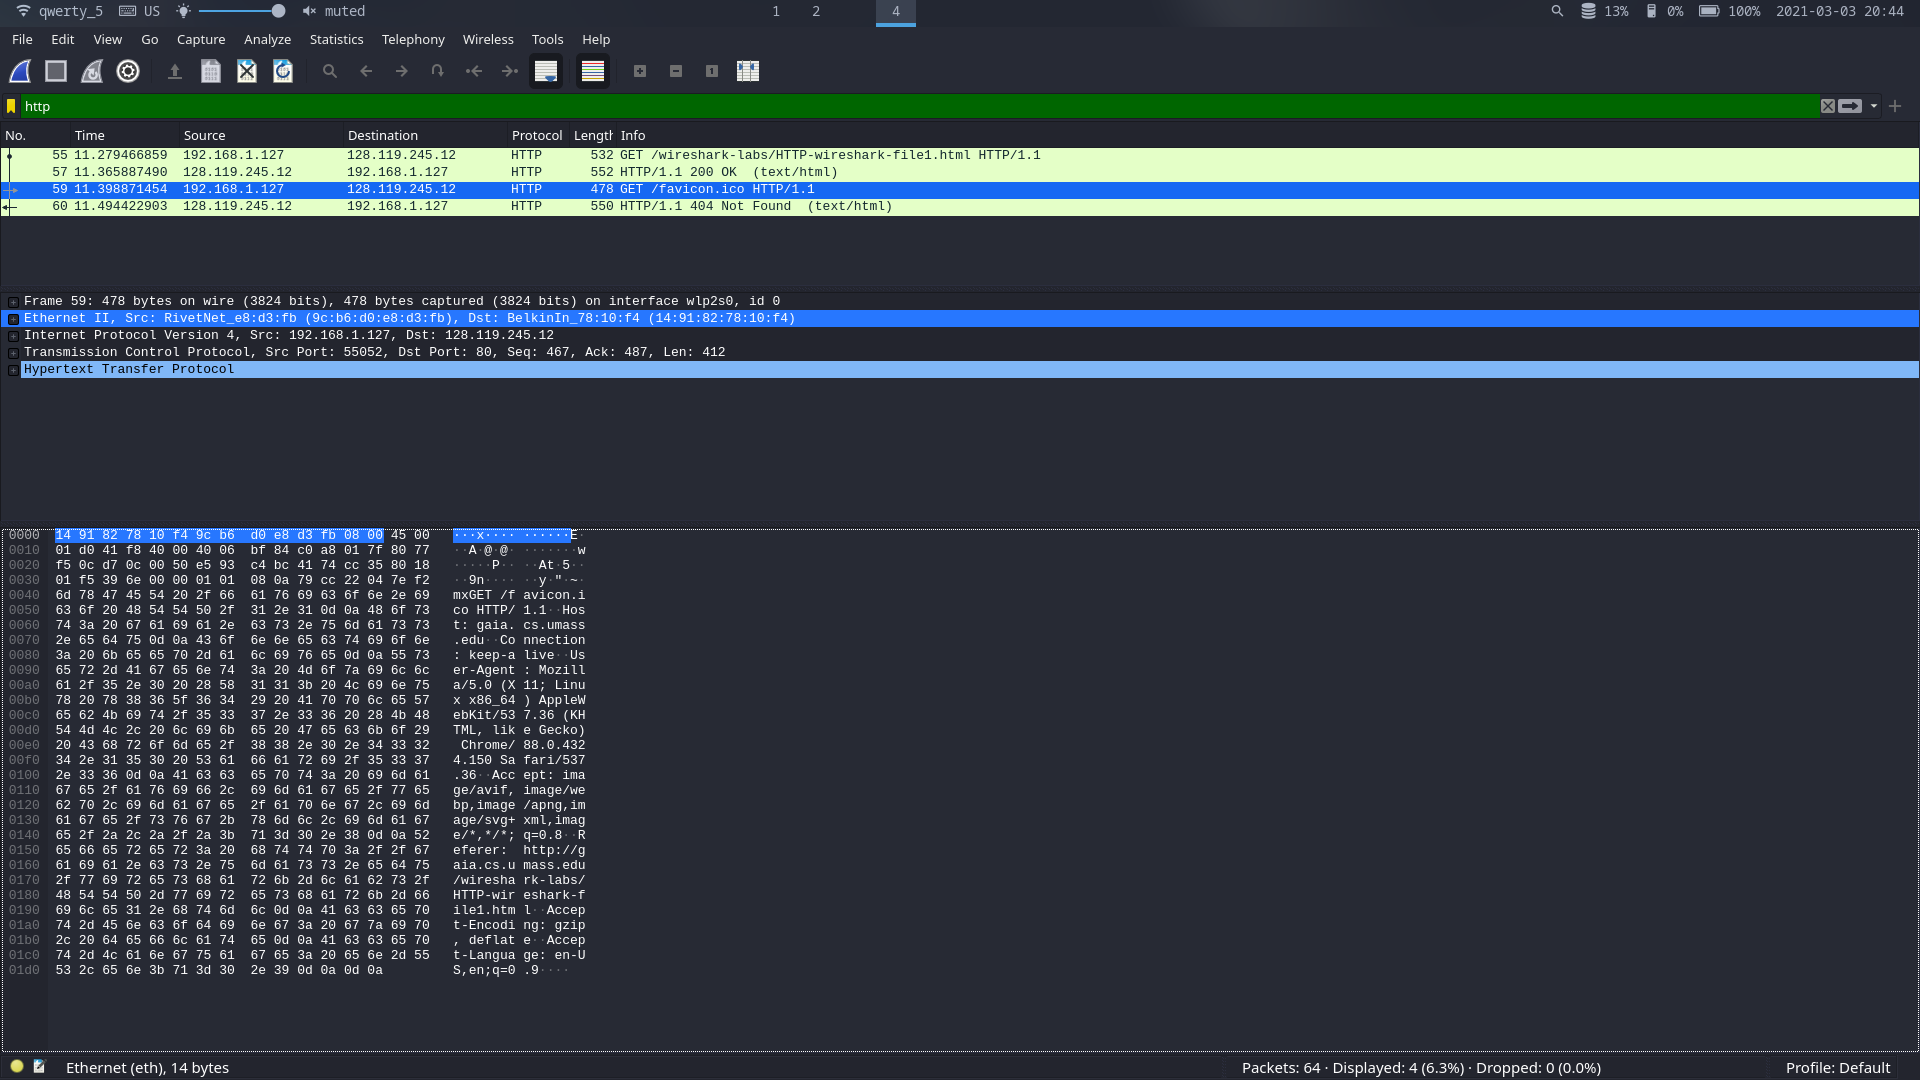
\includegraphics[width=\textwidth]{img/ws-raw-data-3}
  \item 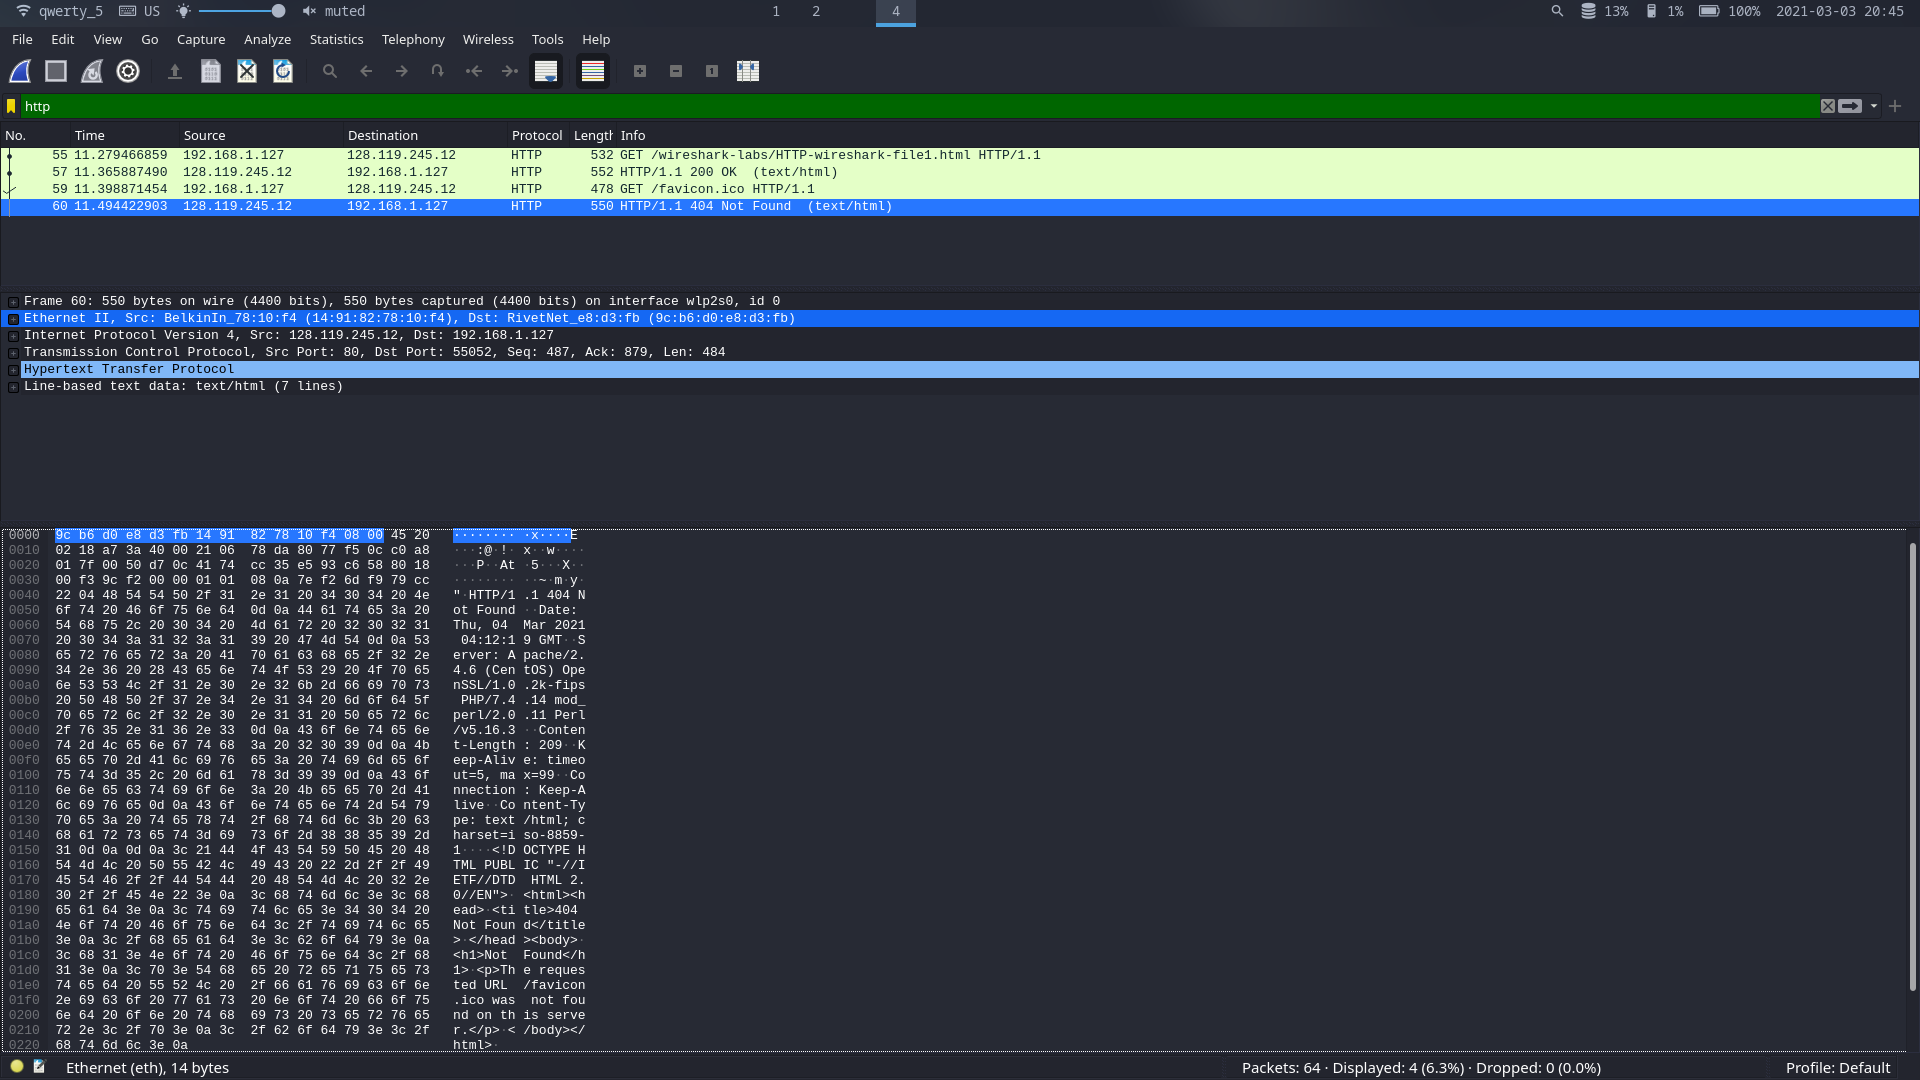
\includegraphics[width=\textwidth]{img/ws-raw-data-4}
  \end{itemize}
\end{enumerate}

\subsection{The HTTP CONDITIONAL GET/response interaction}

\begin{enumerate}
  \setcounter{enumi}{7}
\item Inspect the contents of the first HTTP GET request from your browser to
  the server.  Do you see an ``IF-MODIFIED-SINCE'' line in the HTTP GET?
  \begin{itemize}
  \item I do not see an ``IF-MODIFIED-SINCE'' line in the HTTP GET.\
  \item 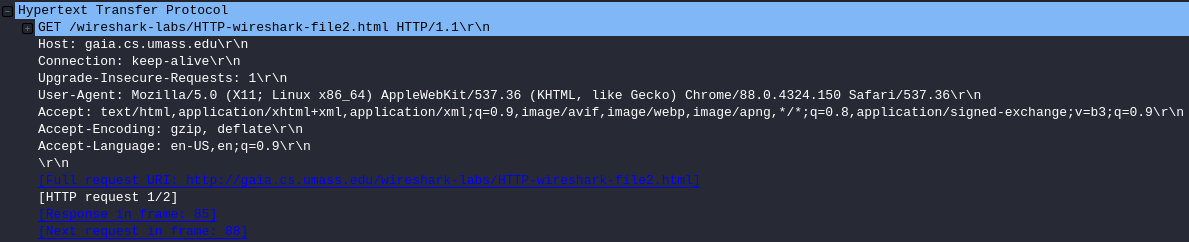
\includegraphics[width=\textwidth]{img/ws-if-modified-since-1}
  \end{itemize}
\item Inspect the contents of the server response. Did the server explicitly
  return the contents of the file?  How can you tell?
  \begin{itemize}
  \item The server explicitly returned the contents.  I can tell because the
    response contains the HTML file content, and content fields like
    ``Content-Type'' and ``Content Length'' are set.
  \item 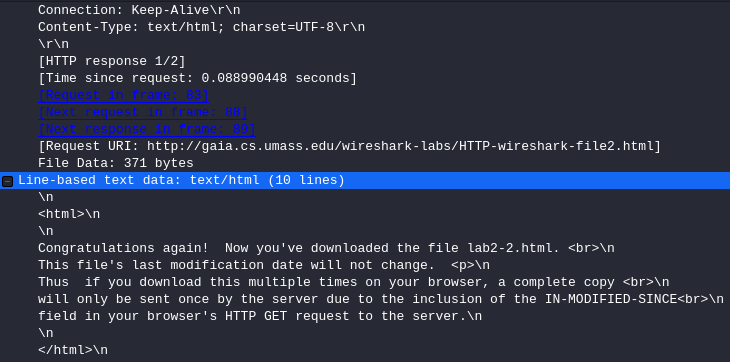
\includegraphics[width=\textwidth]{img/ws-html-contents}
  \item 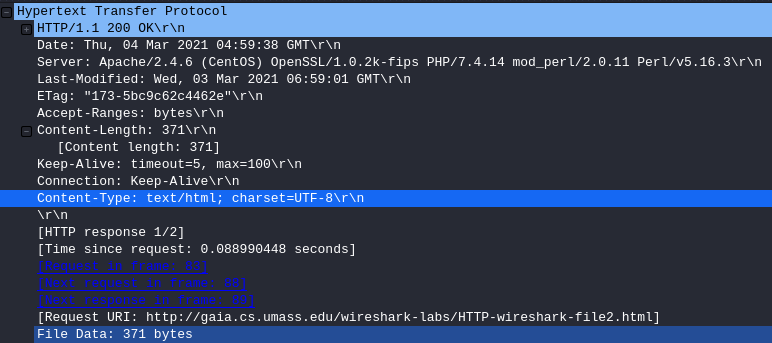
\includegraphics[width=\textwidth]{img/ws-html-content-type}
  \end{itemize}
\item Now inspect the contents of the second HTTP GET request from your browser
  to the server.  Do you see an ``IF-MODIFIED-SINCE:'' line in the HTTP GET?  If
  so, what information follows the ``IF-MODIFIED-SINCE:'' header?
  \begin{itemize}
  \item There is an ``If-Modified-Since'' line, and it contains ``Wed, 03 Mar
    2021 06:59:01 GMT''.
  \item 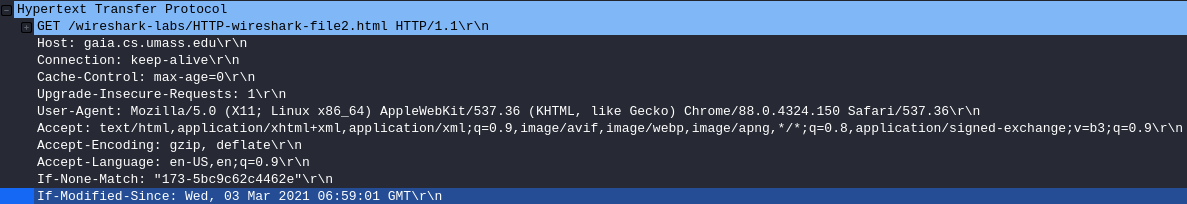
\includegraphics[width=\textwidth]{img/ws-if-modified-since-2}
  \end{itemize}
\item What is the HTTP status code and phrase returned from the server in
  response to this second HTTP GET?  Did the server explicitly return the
  contents of the file?
  \begin{itemize}
  \item The HTTP status code is $304$ and the response phrase is ``Not
    Modified''.  The server did not explicitly return the contents of the file,
    as none of the signs described in the response to question 9 appeared
    here.
  \item 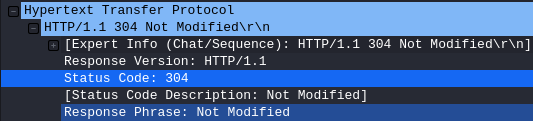
\includegraphics[width=\textwidth]{img/ws-conditional-status-phrase}
  \end{itemize}
\end{enumerate}

\subsection{Retrieving Long Documents}

\begin{enumerate}
  \setcounter{enumi}{11}
\item How many HTTP GET request messages did your browser send?  Which packet
  number in the trace contains the GET message for the Bill or Rights?
  \begin{itemize}
  \item My browser sent one HTTP GET request.  The packet number was $63$.
  \item 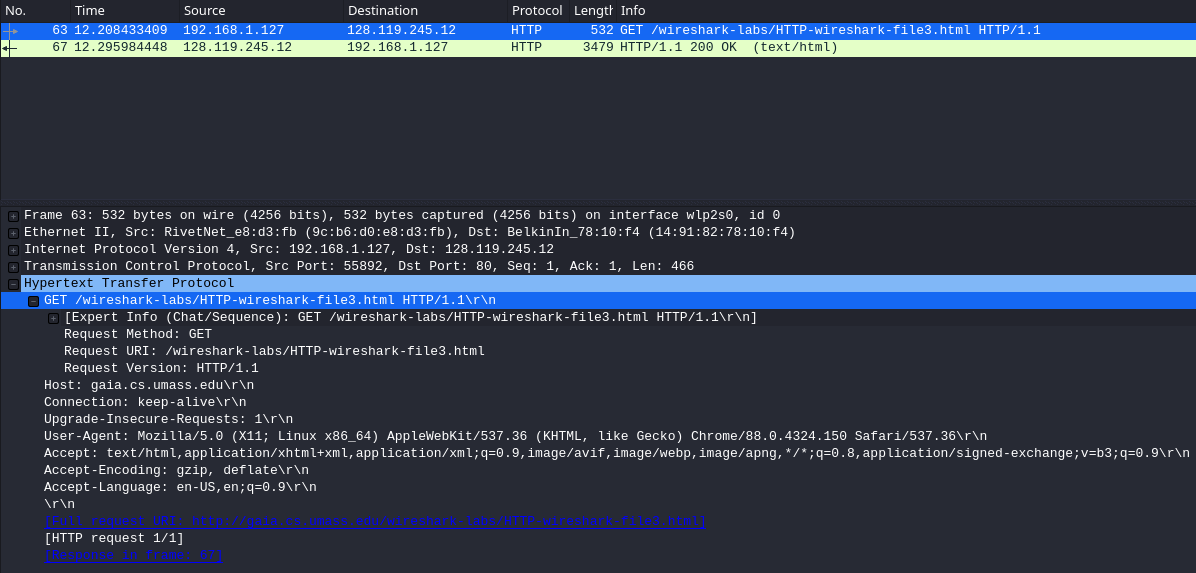
\includegraphics[width=\textwidth]{img/ws-long-get}
  \end{itemize}
\item Which packet number in the trace contains the status code and phrase
  associated with the response to the HTTP GET request?
  \begin{itemize}
  \item The packet number is $65$.  We see that the response was broken into $2$
    TCP segments.  The raw data of the first segment, packet $65$, is
    highlighted in blue, and we see the HTTP status code and phrase at the top
    of the raw data.
  \item 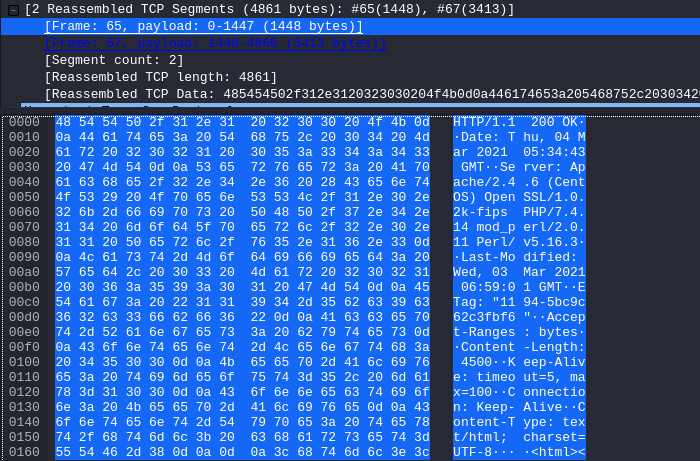
\includegraphics[width=\textwidth]{img/ws-packet-number-long-doc}
  \end{itemize}
\item What is the status code and phrase in the response?
  \begin{itemize}
  \item The status code is $200$, and the phrase is ``OK''.
  \item 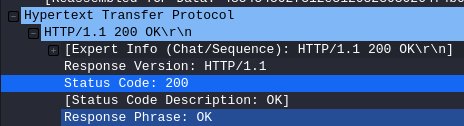
\includegraphics[width=\textwidth]{img/ws-long-doc-status-code-phrase}
  \end{itemize}
\item How many data-containing TCP segments were needed to carry the single HTTP
  response and the text of the Bill of Rights?
  \begin{itemize}
  \item $2$ data-containing TCP segments were needed.
  \item 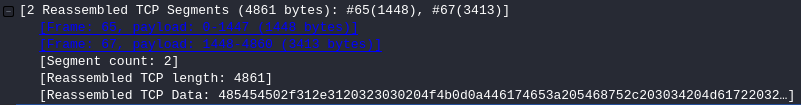
\includegraphics[width=\textwidth]{img/ws-long-doc-tcp-count}
  \end{itemize}
\end{enumerate}

\subsection{HTML Documents with Embedded Objects}

\begin{enumerate}
  \setcounter{enumi}{15}
\item How many HTTP GET request messages did your browser send?  To which
  Internet addresses were these GET requests sent?
  \begin{itemize}
  \item $3$ HTTP GET requests were sent.  The first two went to
    128.119.245.12 (\texttt{gaia.cs.umass.edu}), while the third went to
    178.79.137.164 (\texttt{kurose.cslash.net}).
  \item 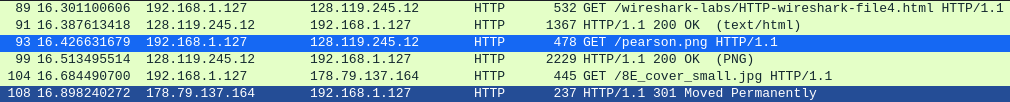
\includegraphics[width=\textwidth]{img/ws-embed-get-count}
  \item 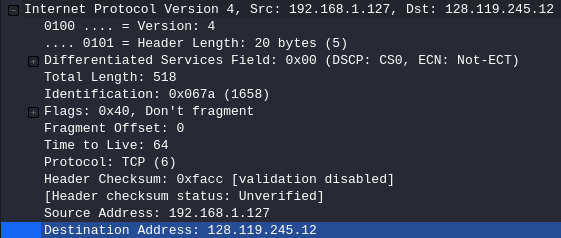
\includegraphics[width=\textwidth]{img/ws-embed-ip-1}
  \item 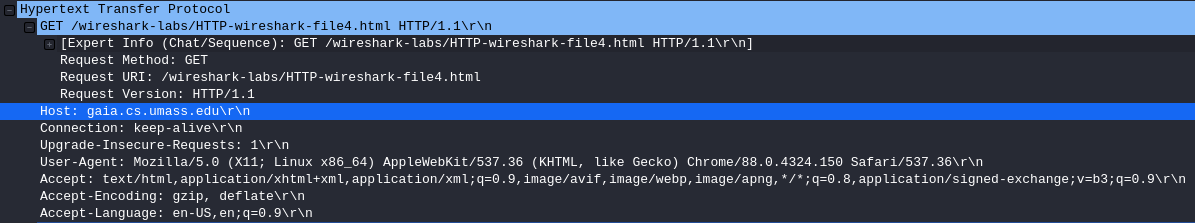
\includegraphics[width=\textwidth]{img/ws-embed-host-1}
  \item 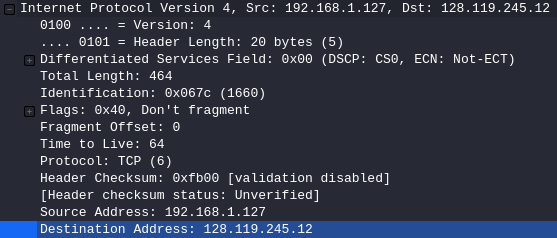
\includegraphics[width=\textwidth]{img/ws-embed-ip-2}
  \item 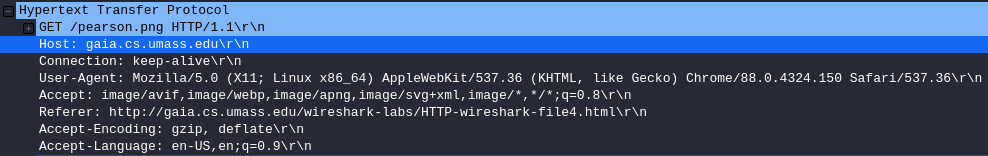
\includegraphics[width=\textwidth]{img/ws-embed-host-2}
  \item 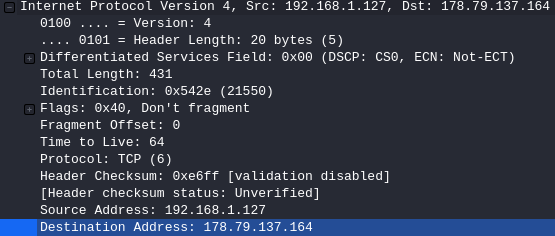
\includegraphics[width=\textwidth]{img/ws-embed-ip-3}
  \item 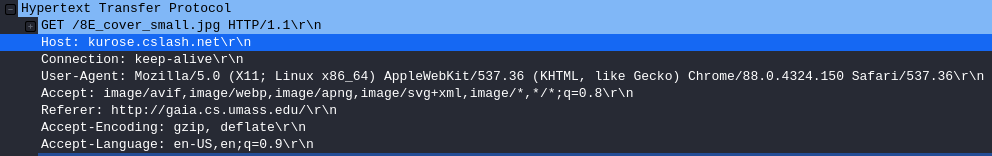
\includegraphics[width=\textwidth]{img/ws-embed-host-3}
  \end{itemize}
\item Can you tell whether your browser downloaded the two images serially, or
  whether they were downloaded from the two web sites in parallel?  Explain.
  \begin{itemize}
  \item The images were downloaded serially.  The last packet for
    \texttt{pearson.png} (packet $99$) arrived before the GET request for
    \texttt{8E\_cover\_small.jpg} (packet $104$) was sent.
  \item 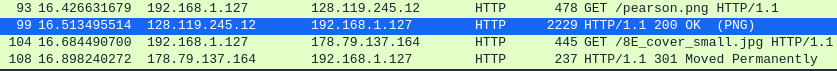
\includegraphics[width=\textwidth]{img/ws-embed-order}
  \end{itemize}
\end{enumerate}

\subsection{HTTP Authentication}

\begin{enumerate}
  \setcounter{enumi}{17}
\item What is the server’s response (status code and phrase) in response to the
  initial HTTP GET message from your browser?
  \begin{itemize}
  \item The server responded with $401$ and ``Unauthorized''.
  \item 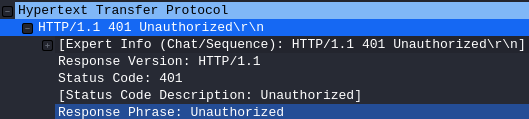
\includegraphics[width=\textwidth]{img/ws-auth-1}
  \end{itemize}
\item When your browser’s sends the HTTP GET message for the second time, what
  new field is included in the HTTP GET message?
  \begin{itemize}
  \item The ``Authorization'' and ``Cache-Control'' fields are new.
  \item 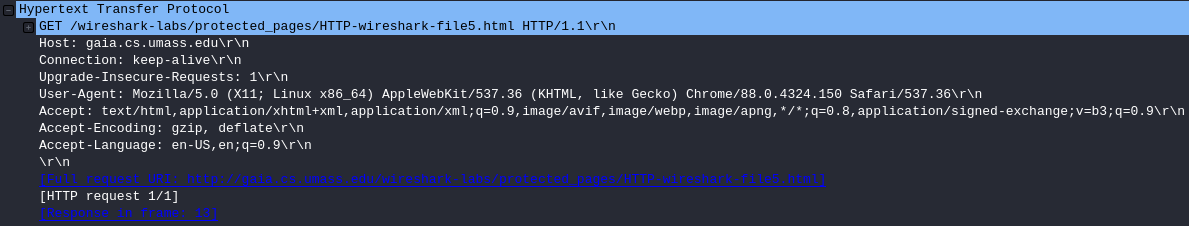
\includegraphics[width=\textwidth]{img/ws-auth-new-fields-1}
  \item 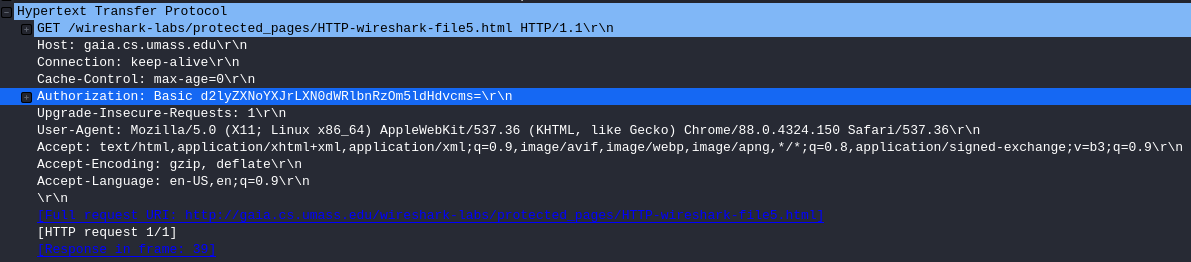
\includegraphics[width=\textwidth]{img/ws-auth-new-fields-2}
  \end{itemize}
\end{enumerate}


\break
\section{Web Proxy Cache}
    This TCP Proxy Server stores its cached websites in a local directory that gets created inside the working directory of the program when the first request is accepted and processed. The main loop waits for the TCP server to receive a client request and has a timeout of 1 second. Its in a try catch nested in an infinite loop to enable the user to interrupt the program with a keyboard interrupt like "ctrl+c". Without implementing this loop and putting a timeout on the TCP Server socket, the proxy server has to be forcubly shut down because the sockets are blocking. When a request is received from the client, a client server socket is generated directly from the tcpServSock.accept() function. The message is then decoded and the url, filename and host are extracted from the message. The program then checks the "cached" directory to see if the received file request already exists.\\ 
    
    If it exists, the request does not get forwarded to the host server and instead simply responds with the contents of the locally cached file. This cached response shows significantly increased response speeds as compared to true requests from host servers. The responses are stored locally in files, so restarting the program or your computer will not destroy the cached files. They have to either be deleted manually or by the program when it starts. \\
    
    If the file does not exist in the local cache, a new socket is created on the Proxy Server and connected to the host domain on port 80. A new request is built using  the filename and host previously extracted from the client request message. The message is sent in the form "GET \textit{filename} HTTP/1.1 Host: \textit{hostDomain} Connection: Close". The "Close" connection is to force the connection to close rather then the default "keep\_open" Connection type. Once this message is built  and sent to the host, the socket waits until it receives a response. Once received, the response is first sent back to the client server to reduce the delay, then the response is stored in a local file in the "cached" directory using the same "filename". Once the message has been both stored in the final and sent to the client then host and client sockets are shutdown and the process repeats. \\
    
    I have also ensured proper exception handling and a way to compare cached vs noncached times. The times are compared using a dictionary that is created on program run. It stores the time it takes to send a response to the client from the point the connection is created between the client and proxy until a response message is sent using the requests filename as a key. When the server is killed, the results of this dictionary are printed to the console. A bar graph comparing load times can be seen below. \\

\begin{figure}
    \centering
    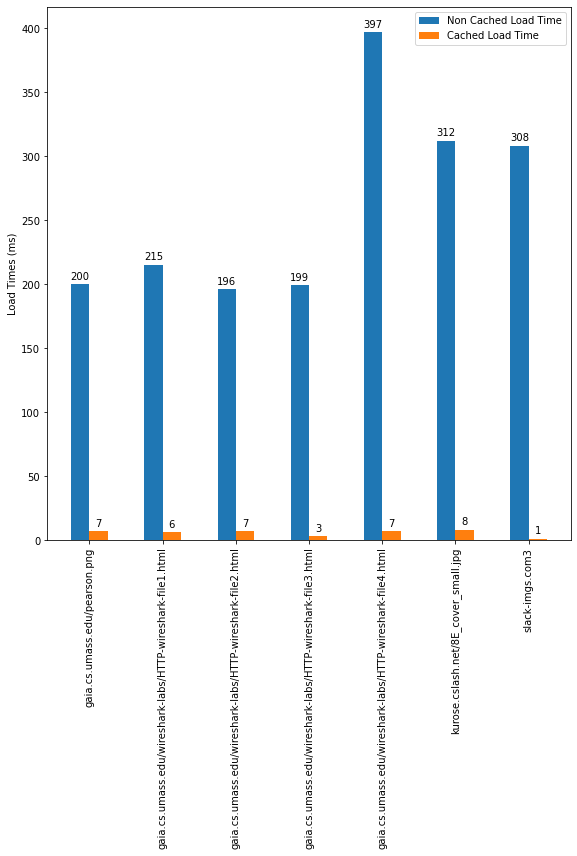
\includegraphics[width=0.8\textwidth]{img/proxy_server_load_times_graph.png}
    \caption{Proxy Server Load Times for Cached and Non Cached Requests}
    \label{fig:my_label}
\end{figure}

\begin{center}
  \item 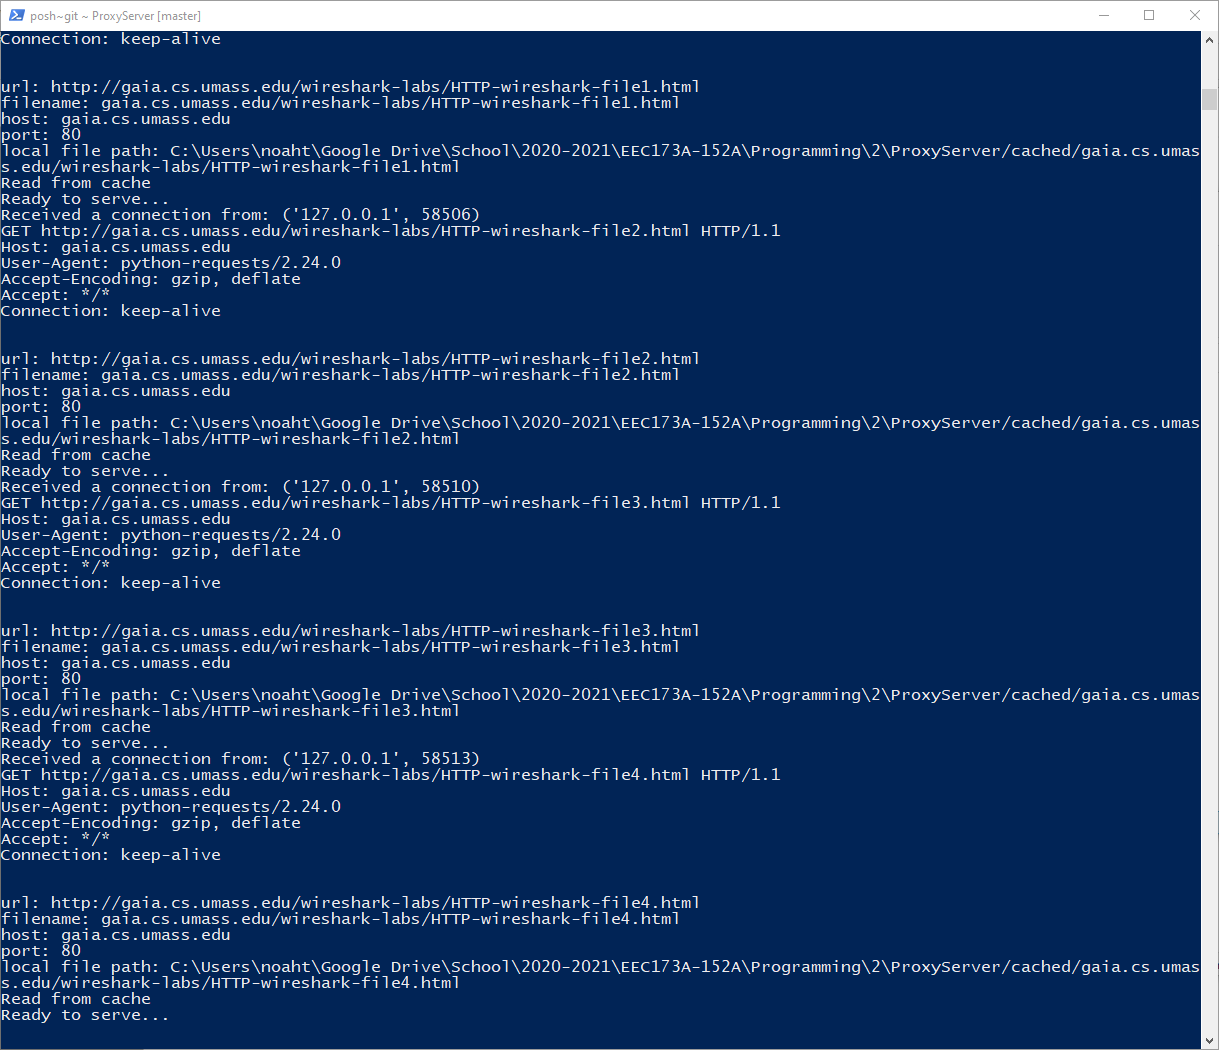
\includegraphics[width=0.8\textwidth]{img/proxy_server_terminal.PNG}
  \item 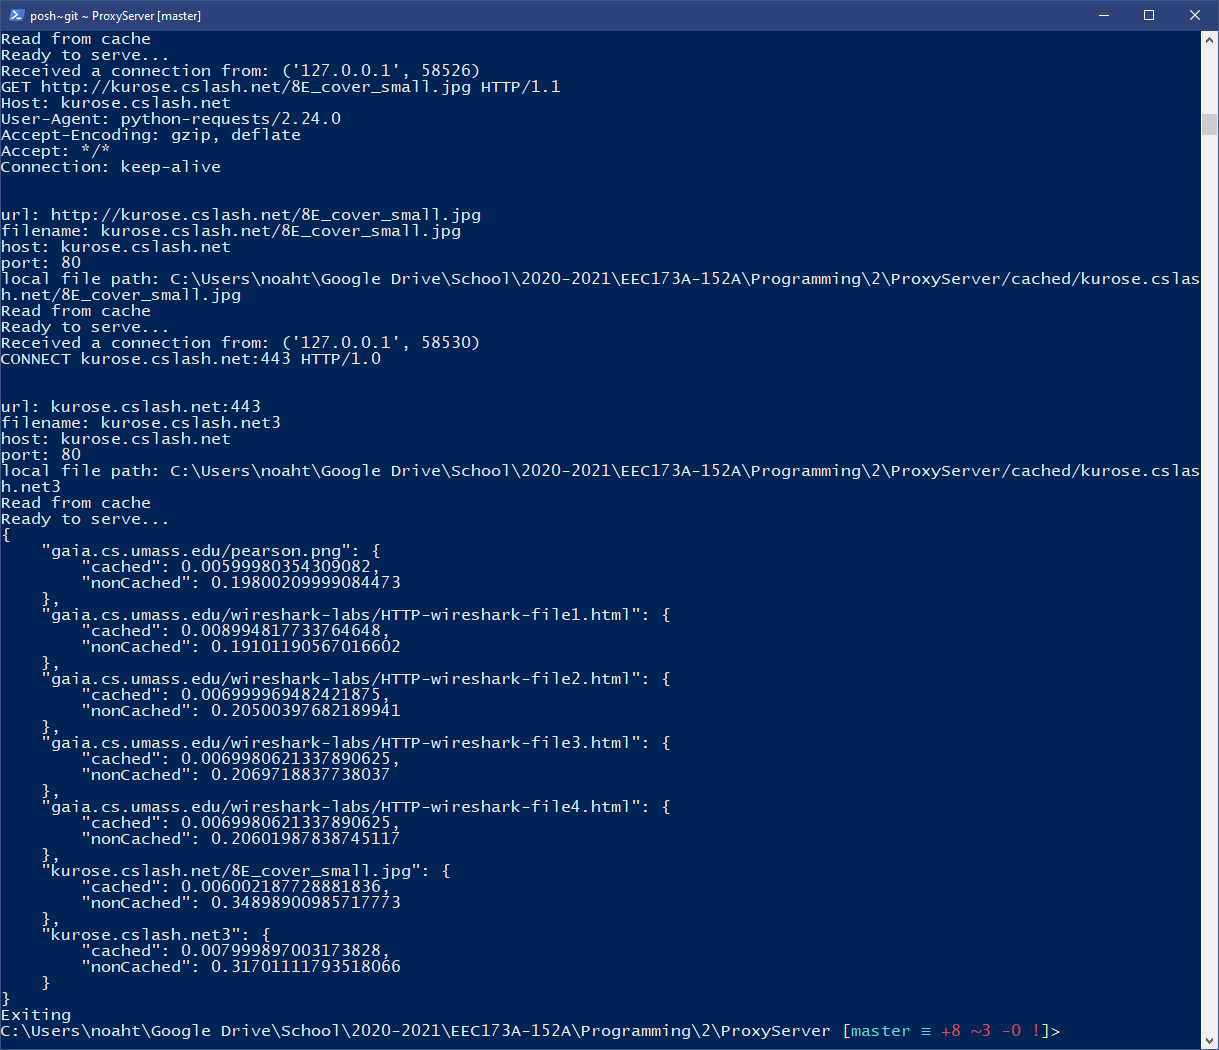
\includegraphics[width=0.8\textwidth]{img/proxy_server_terminal_on_exit.PNG}
  \break
  \item 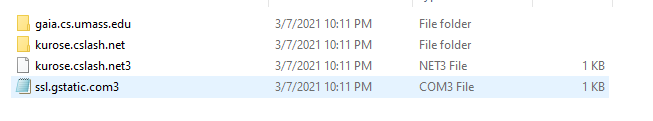
\includegraphics[width=0.8\textwidth]{img/local_cached_directory.PNG}
  \item 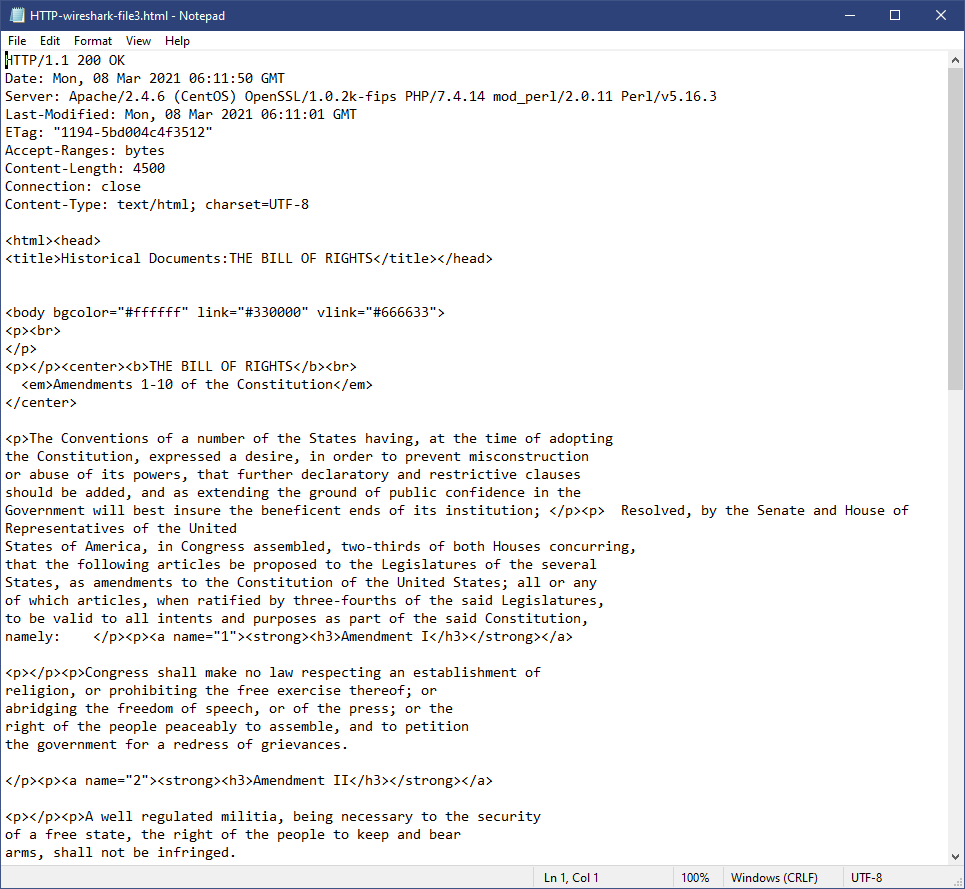
\includegraphics[width=0.8\textwidth]{img/cached_website_html_code.PNG}
\end{center}

\break
\section{DNS and \texttt{dig}}

\begin{enumerate}[label=(\alph*)]
\item Starting with a root DNS server (from one of the root servers
  [a-m].root-servers.net), initiate a sequence of queries for the IP address for
  your department’s Web server by using dig. Show the list of the names of DNS
  servers in the delegation chain in answering your query.
  \begin{itemize}
  \item I followed the DNS servers \texttt{a.root-servers.net} $\rightarrow$
    \texttt{a.edu-servers.net} $\rightarrow$ \texttt{dns-two.ucdavis.edu}.  The IP
    addresses are listed in the last screenshot under ``ANSWER SECTION''.
  \item 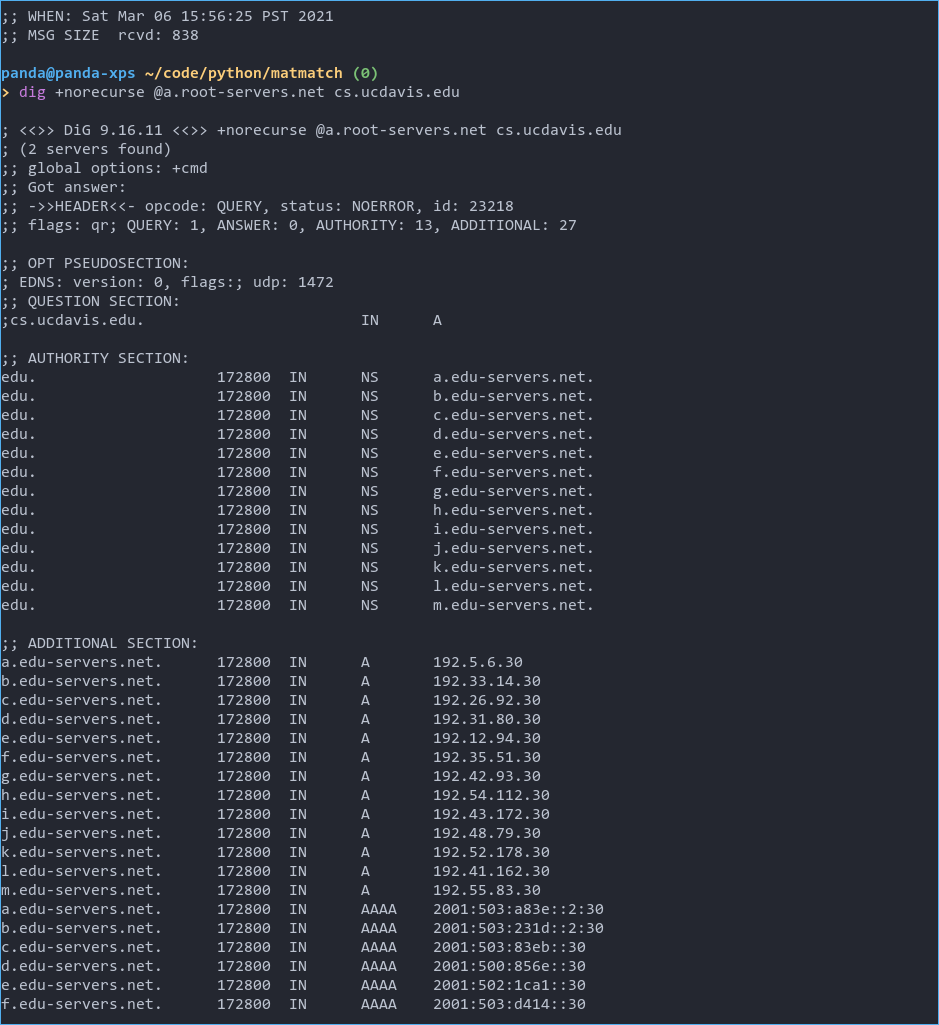
\includegraphics[width=0.7\textwidth]{img/dig-ucd-1}
  \item 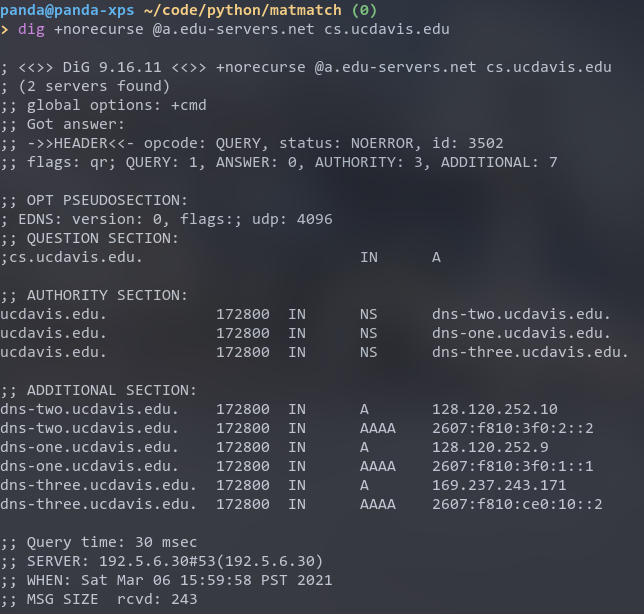
\includegraphics[width=0.7\textwidth]{img/dig-ucd-2}
  \item 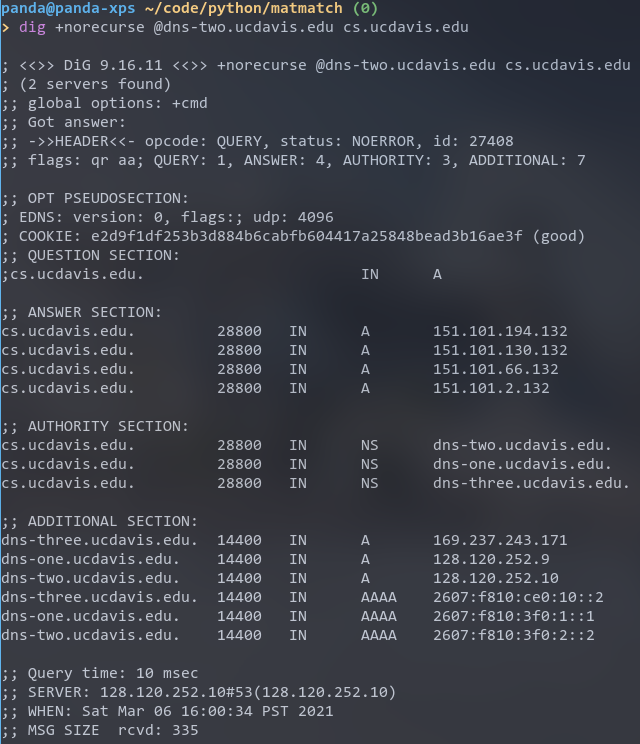
\includegraphics[width=0.7\textwidth]{img/dig-ucd-3}
  \end{itemize}
\item Repeat part (a) for several popular Web sites, such as google.com,
  yahoo.com, or amazon.com
  \begin{itemize}
  \item google.com
    \begin{itemize}
    \item I followed the DNS servers \texttt{a.root-servers.net} $\rightarrow$
      \texttt{a.gtld-servers.net} $\rightarrow$ \texttt{ns2.google.com} to get
      the IP address 216.58.194.174.
    \item 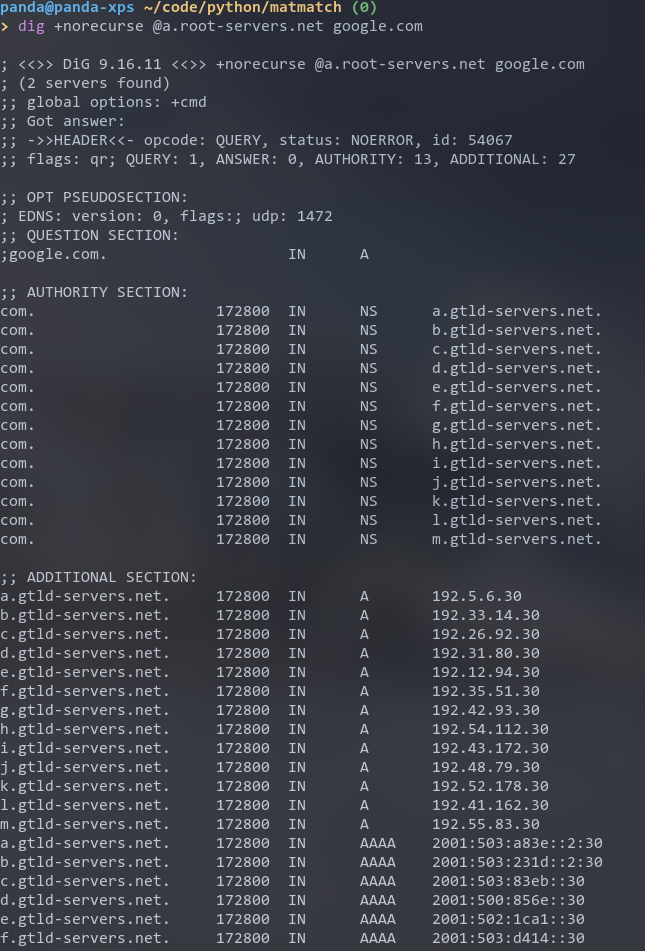
\includegraphics[width=0.7\textwidth]{img/dig-google-1}
    \item 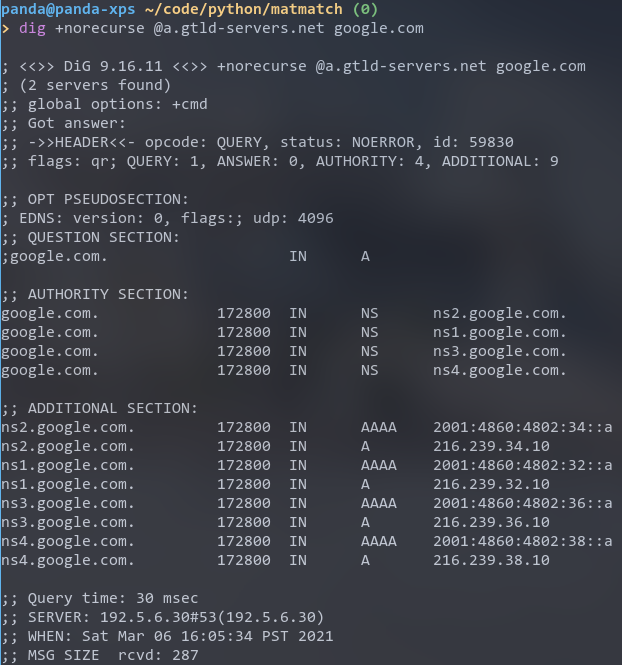
\includegraphics[width=0.7\textwidth]{img/dig-google-2}
    \item 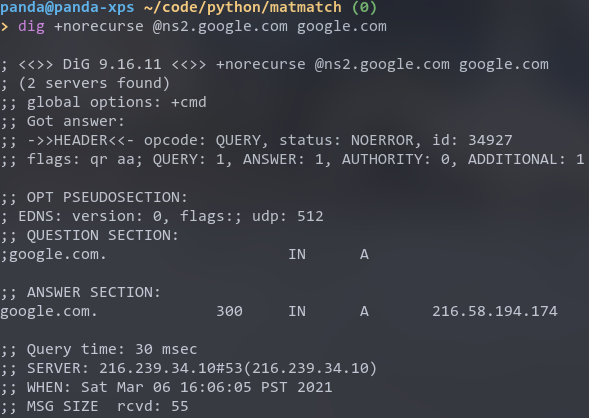
\includegraphics[width=0.7\textwidth]{img/dig-google-3}
    \end{itemize}
  \item yahoo.com
    \begin{itemize}
    \item I followed the DNS servers \texttt{a.root-servers.net} $\rightarrow$
      \texttt{a.gtld-servers.net} $\rightarrow$ \texttt{ns1.yahoo.com}.  The IP
      addresses are listed in the last screenshot under ``ANSWER SECTION''.
    \item 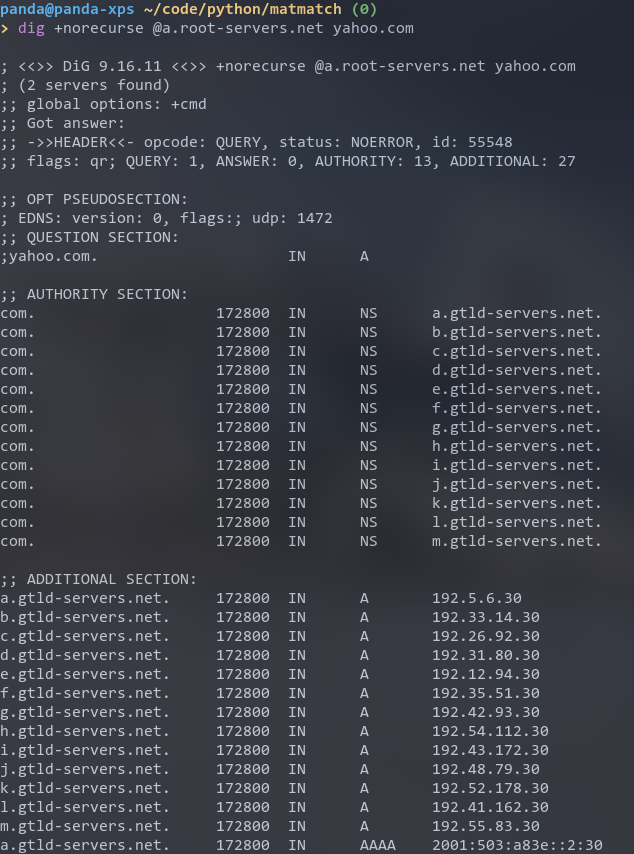
\includegraphics[width=0.7\textwidth]{img/dig-yahoo-1}
    \item 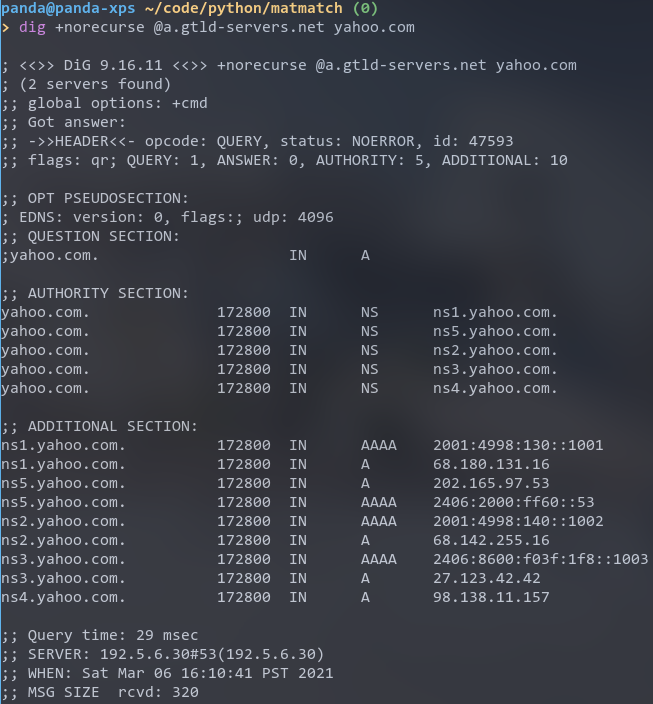
\includegraphics[width=0.7\textwidth]{img/dig-yahoo-2}
    \item 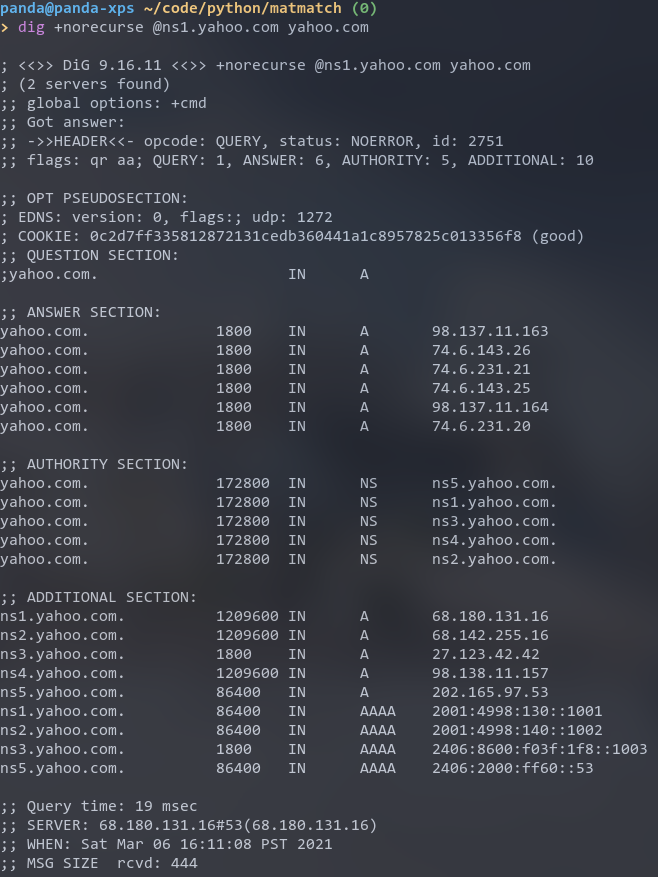
\includegraphics[width=0.7\textwidth]{img/dig-yahoo-3}
    \end{itemize}
  \item github.com
    \begin{itemize}
    \item I followed the DNS servers \texttt{a.root-servers.net} $\rightarrow$
      \texttt{e.gtld-servers.net} $\rightarrow$ \texttt{ns-520.awsdns-01.net} to get
      the IP address 192.30.255.112.
    \item 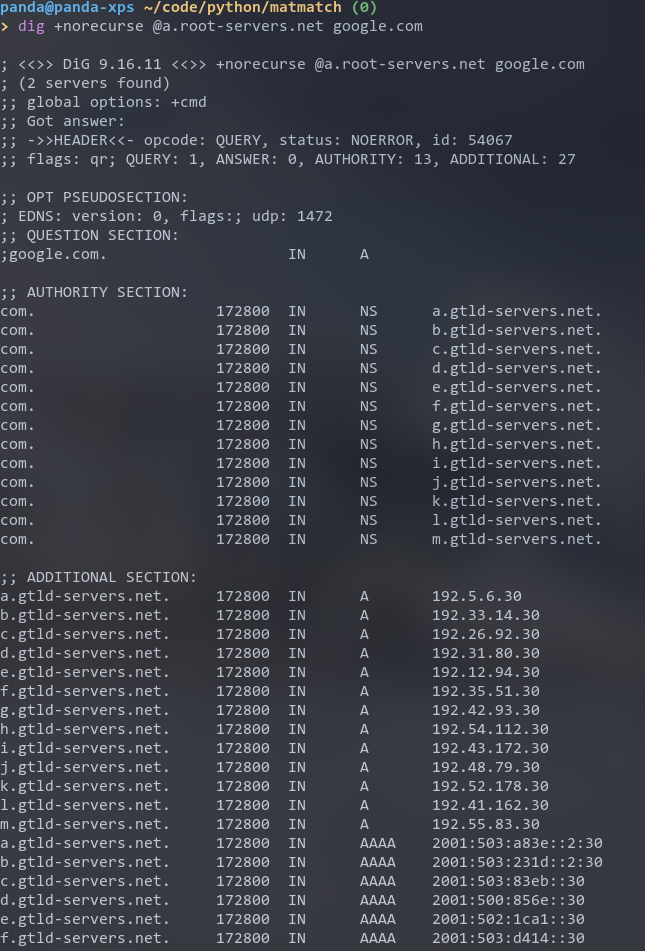
\includegraphics[width=0.7\textwidth]{img/dig-google-1}
    \item 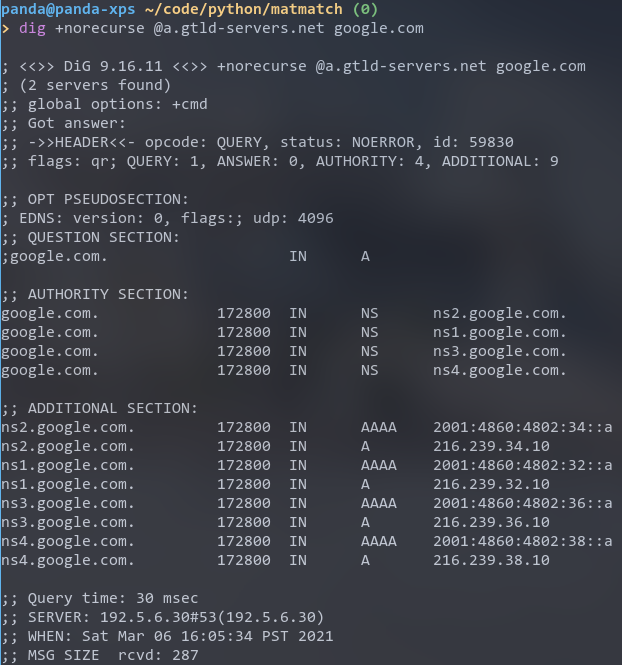
\includegraphics[width=0.7\textwidth]{img/dig-google-2}
    \item \includegraphics[width=0.7\textwidth]{img/dig-google-3}
    \end{itemize}
  \item messenger.com
    \begin{itemize}
    \item I followed the DNS servers \texttt{a.root-servers.net} $\rightarrow$
      \texttt{e.gtld-servers.net} $\rightarrow$ \texttt{a.ns.facebook.com} to get
      the IP address 69.171.250.15.
    \item \includegraphics[width=0.7\textwidth]{img/dig-messenger-1}
    \item \includegraphics[width=0.7\textwidth]{img/dig-messenger-2}
    \item \includegraphics[width=0.7\textwidth]{img/dig-messenger-3}
    \end{itemize}
  \item whitehouse.gov
    \begin{itemize}
    \item I followed the DNS servers \texttt{a.root-servers.net} $\rightarrow$
      \texttt{a.gov-servers.net} $\rightarrow$ \texttt{use6.akam.net} to get
      the IP address 23.219.242.151.
    \item \includegraphics[width=0.7\textwidth]{img/dig-whitehouse-1}
    \item \includegraphics[width=0.7\textwidth]{img/dig-whitehouse-2}
    \item \includegraphics[width=0.7\textwidth]{img/dig-whitehouse-3}
    \end{itemize}
  \end{itemize}
\end{enumerate}

\end{document}
